\documentclass[tikz]{standalone}

\usepackage[utf8]{inputenc}
\usepackage[T1]{fontenc}
\usepackage{cmap}
\usepackage{amsmath}
\usepackage{amssymb}
\usepackage{verbatim}
\usepackage{bm}
\usepackage{siunitx}

\renewcommand{\familydefault}{\sfdefault}
\usepackage[cm]{sfmath}


\usepackage{tikz}
\usetikzlibrary{math}
\usetikzlibrary{bending}
\usetikzlibrary{decorations.pathreplacing}
\usetikzlibrary{decorations.pathmorphing}
\definecolor{cblue}{rgb}{0.396, 0.643, 0.82}
\definecolor{corange}{rgb}{1.0, 0.69, 0.416}

\def\symbhwaas{N_a}
\def\symbsteplen{\Delta d}
\def\symbsweeprate{f_s}
\def\symbsweepperiod{T_s}
\def\symbsweepdur{\tau_s}
\def\symbframerate{f_f}
\def\symbframeperiod{T_f}
\def\symbframedur{\tau_f}
\def\symbprf{f_\text{p}}
\def\symbspf{N_s}
\def\symbstartpoint{d_1}
\def\symbnumpoints{N_d}
\def\symbmur{r_\text{u}}
\def\symbcid{r_\ell}
\def\symbminmd{r_\text{min}}
\def\symbmaxmd{r_\text{max}}
\def\symbdcrnear{r_\text{near}}
\def\symbdcrfar{r_\text{far}}

\begin{document}

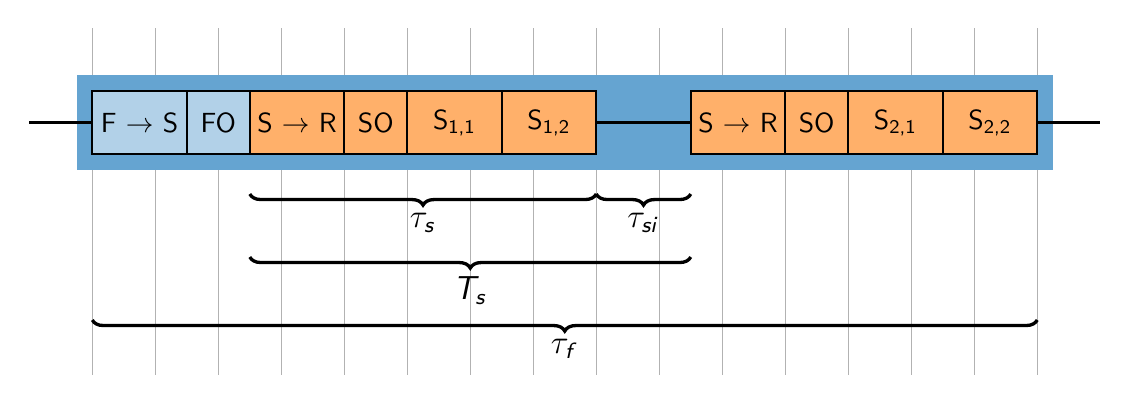
\begin{tikzpicture}[scale=0.8]
  \tikzmath{}

  \draw [thin, black!30, ystep=0] (1, -4) grid (16, 1.5);

  \fill [fill=cblue] (0.75, -0.75) rectangle ++(15.5, 1.5);

  \draw [very thick] (0, 0) -- ++(17, 0);

  \draw [fill=cblue!50, thick] (1, -0.5) rectangle ++(1.5, 1) node[midway] {F $\rightarrow$ S};
  \draw [fill=cblue!50, thick] (2.5, -0.5) rectangle ++(1, 1) node[midway] {FO};

  \draw [fill=corange, thick] (3.5, -0.5) rectangle ++(1.5, 1) node[midway] {S $\rightarrow$ R};
  \draw [fill=corange, thick] (5, -0.5) rectangle ++(1, 1) node[midway] {SO};
  \draw [fill=corange, thick] (6, -0.5) rectangle ++(1.5, 1) node[midway] {$\text{S}_{1,1}$};
  \draw [fill=corange, thick] (7.5, -0.5) rectangle ++(1.5, 1) node[midway] {$\text{S}_{1,2}$};

  \draw [fill=corange, thick] (10.5, -0.5) rectangle ++(1.5, 1) node[midway] {S $\rightarrow$ R};
  \draw [fill=corange, thick] (12.0, -0.5) rectangle ++(1, 1) node[midway] {SO};
  \draw [fill=corange, thick] (13.0, -0.5) rectangle ++(1.5, 1) node[midway] {$\text{S}_{2,1}$};
  \draw [fill=corange, thick] (14.5, -0.5) rectangle ++(1.5, 1) node[midway] {$\text{S}_{2,2}$};

  \draw [very thick, decoration={brace, amplitude=4pt, mirror, raise=3pt}, decorate] (3.5, -1) -- node[below=6pt] {\large $\tau_s$} ++(5.5, 0);
  \draw [very thick, decoration={brace, amplitude=4pt, mirror, raise=3pt}, decorate] (9, -1) -- node[below=6pt] {\large $\tau_{si}$} ++(1.5, 0);

  \draw [very thick, decoration={brace, amplitude=4pt, mirror, raise=3pt}, decorate] (3.5, -2) -- node[below=6pt] {\large $T_s$} ++(7, 0);

  \draw [very thick, decoration={brace, amplitude=4pt, mirror, raise=3pt}, decorate] (1, -3) -- node[below=6pt] {\large $\tau_f$} ++(15, 0);

\end{tikzpicture}

\end{document}
